Um sistema multiagente(SMA) organizado é aquel constituido por agentes autonomos que interagem visando um propósito em comum tendo como consequência um comportamento global \cite{mosieframework} 
\cite{organiationofmultiagentsystem}. Assim sendo, uma organização com essas características deve ser capaz de manifestar conhecimento em comum, cultura, memória, história, distribuição de atividades 
e a capaciade de distinguir um  agente em espeçifico \cite{organiationofmultiagentsystem}. Deste fato é possível identificar o fenômeno "supra-individual" que implica em um comportamento que existe
além dos comportamentos e atributos particulares no que diz respeito as entidades constituintes do sistemas. 

Uma organização de um sistema multiagente deve conter relações sociais no que tange a agentes, institutos e grupos sociais \cite{organiationofmultiagentsystem}. Ainda sobre isso, uma organização 
\textit{SMA} deve apresentar uma \textit{extensão de um espaço abstrato}. Isso implica uma representação dos seguintes conceitos; estrutra espacial, estrutura temporal, símbolos, semântica e 
capacidade de dedução. Há organizações que não se enquadram em todas essas restrições, contudo são suficientes para tratar o problema dentro de uma perspectiva computacional \cite{organiationofmultiagentsystem}.

O subtópico \textit{Conceitos Gerais de uma Organização de Siastems Multiagentes} tem como por finalidade detalhar melhor os elementos presentes da Teoria da Organização dentro do contexto de SMA
em relação a esse estudo. Já o Subtópico \textit{Formalização de Conceitos Específicos para SMA} tem como por objetivo realizar uma verificação analítica dos elementos presentes no modelo de \textit{SMA} 
denomiando por \textit{MOISE+}. Os conceitos que serão analisados são; objetivos, planos e papeis \textit{organiationofmultiagentsystem}.
   

\subsection{Conceitos Gerais de uma Organização de Sistemas Multiagentes}

A finalidade desta subseção consiste trabalhar com uma maior riqueza de detalhes todos os conceitos que constituem a ideia de uma organiozação de um sistema multiagente.  
  
\textbf{Divisão em tipos de atividades:} Uma organização não é uniformemente estruturada. Isso, pois as atividades são distribuidas de forma desigual entre as diferentes entidades.
Dentro do ponto de vista fenomenologico as atividades são sujeitas a classificação e ocorrem com diferentes frequências e em diferentes regiões dentro das definições espaciais da organização \cite{organiationofmultiagentsystem}.

\textbf{Integração:} Dentro de uma organização ocorre a presenção de interdependência entre diferentes espaços de ativiades. Essas, por sua vez, estão relacionadas em uma estrutura única definida
dentro de um contexto alinhado e integrado \cite{organiationofmultiagentsystem}.

\textbf{Composição} Uma organnização é composta por elementos menores. No caso dos multiagentes, os elementos atomicos que estruturam a organização são os agentes \cite{organiationofmultiagentsystem}.

\textbf{Estabilidade/Flexibilidade:} Uma organização apresenta padrões de atividades. Esses padrões possum cateristicas que podem ser enquadradas em dois aspectos; estaveis e flexiveis. 
No que tange as características estaveis, essas são constituidas por elementos/processos que definem o padrão em sí mesmo. Em constraste com isso um comportamento flexível acontece quando o 
sistema é submetido a situações incomuns \cite{organiationofmultiagentsystem} \textbf{?}.

\textbf{Coordenação:} Todo sistema é dependente de algum dado recurso. Assim sendo, se faz necessário que esse recurso seja utilizado de forma inteligente a fim de que possa se manter ao longo 
do tempo. Para que isso, se faz necessário que a organização se comporte como uma amplificadora de recursos a fim de que as estruturas operacionais tenham um comportamente cada vez mais organizado 
\cite{selforganization}, \cite{selforganizatioenvoriment}, \cite{defintionselforganization}. Contudo as incertezas relacioandos aos efeitos combinados resultam
influenciam negativamente nas eficiencias. Portanto, para manter a eficiência organizacional se faz necessário a existência de elementos otimizadores sobre os padrões de atividades \cite{organiationofmultiagentsystem}.

\textbf{Recursividade:} Uma organização é constituída por sub-organizações. Isso ocorre em multiplos níveis de estrutura e se dá por intermédio de um padrão recursivo \cite{organiationofmultiagentsystem}.

\textbf{Representação Multi-Nível e Causaldiade:} Uma organização é estruturada por suborganizações em diferentes níveis estruturas. Isso, por sua vez, resultam em atividades ocorrendo em 
diferentes escalas espaciais, temporais e estruturais. Como consequencia disto, as cadeias causais presentes em estruturas organizacionais são processos multi-níveis \cite{organiationofmultiagentsystem}.

\textbf{Potenciais e Diferenciais:} Diversos são os sistemas físicos onde as forças entre partículas são decorrentes de balanços de potenciais. Como esse comportamento está presente em diversos
sistemas físicos, existe modelos abstratos de sistemas auto-organizaveis que levam em consideração a presença de forças potenciais ediferenciais em organizações \cite{selforganizationdiffforce}. 
Esse conceito é trabalhado dentro de sistemas multiagentes. Um exemplo notório a respeito disto consiste no conceito de \textit{Poder} o qual é entendio como a capacidade de influenciar uma
dada organização \cite{organiationofmultiagentsystem}

\textbf{Regras e Gramáticas:} Organizações podem ser compreendidas como potenciais configurações de atividades e processos. Essas configurações podem ser descritas usando gramática \cite{grammarselforganizationmodel} 
\cite{grammarselforganizationmodel2}. Tanto as gramáticas como as regras que compõem um organização apresentam três interpretações, essas são; como estruturas (especificações procedurais do que deve 
ser feito), como coação as ações defindo o que pode e não pode ser feito e como um compilado das experiênicas \cite{organiationofmultiagentsystem}.

\textbf{Incerteza:} Não é possível conceber o conceito de uma organização sem ao menos entende-la como uma estrutura que distribui informação em sí mesma. Sobre essa ótica, a distrbuição de informação
inequivocamente implica geração de incerteza o que por sua ver se manifesta como um complicante no que tange a comunicação entre as partes bem como a atividade organizacional em si mesma.

\subsection{Formalização de Conceitos Específicos para SMA}

Não há necessidade de usar a ideia de objetivos, planos e papeis para criar um modelo de organização de \textit{SMA}. Isso pois existem formas de criar representações
de \texit{SMA} sem a necessidade de usar esses conceitos \cite{organiationofmultiagentsystem}, \cite{multiagentsystemmodernapproach}. Entretanto, esses conceitos facilitam diversos processos
de especificação, estão presentes em modelos de \textit{SMA} consolidados \cite{mosieframework} e tornam a organização de sistemas multiagentes uma representação mais fidedigna com os processos
sociais presentes na humanidade o que é compartível com os objetivos finais deste estudo. 


A especificação estrutural acontece em três níveis, individual, social e coletivo. O nível individual trata de definir os papeis $\rho$ dos agentes. Uma possível entre os papeis acontece por 
intermédio da hereditariedade em que se $\rho'$ é filho de $\rho$. Isso implica afirmar que $\rho'$ é uma especialização de $\rho$. Um exemplo apropriado para isso é o jogo de futebol onde 
existe o papel jogador dado por $\rho$ e existe o papel atacante dado por $\rho'$ \cite{mosieframework}. Em termos formais, essa relação é dada pro; 
\begin{eqnarray}\nonumber
\rho_a \sqsubset \rho_b
\end{eqnarray}

O nível social estabelece relações de ligação dado pelo predicado $link(\rho_s,\rho_d,t)$. Existe três possíveis valores para $t$, os quais são $t = \{aut, com, acq\}$. O valor $auth$ significa 
autoridade (neste caso $\rho_s$ exerce autoridade sobre $\rho_d$), o valor $com$ significa comunicação (neste caso $\rho_s$ pode se comunicar com $\rho_d$) e o valor $acq$ significa conhecimento 
($\rho_s$ tem conhecimento da existência de $\rho_d$) \cite{mosieframework}. O MOISE+ define as seguintes relações de implicabilidade

\begin{eqnarray}\nonumber
	link(\rho_s,\rho_d,auth) \to link(\rho_s,\rho_d,com) \nonumber \\
	link(\rho_s,\rho_d,com) \to link(\rho_s,\rho_d,acq) 
\end{eqnarray}

O modelo também determina como se dá as relações de hereditariedade para o predicado de $link$, é dado por \cite{mosieframework}; 

\begin{eqnarray}\nonumber
	link(\rho_s,\rho_d,t) \wedge \rho_s' \sqsubset \rho_s' \to link(\rho_s',\rho_d,t) \nonumber \\
	link(\rho_s,\rho_d,t) \wedge \rho_d' \sqsubset \rho_d' \to link(\rho_s,\rho_d',t) 	
\end{eqnarray}


O nível coletivo determina a existência de compatibilidade entre os papeis \cite{mosieframework}. Essa é uma relação reflexiva e transitiva de determina que se um papel $\rho_a$ possui a 
capacidade de realizar um determinado objetivo, então o papel $\rho_b$ também tem essa capacidade. Em termos formais, essa relação se dá da seguinte forma \cite{mosieframework}.;

\begin{eqnarray}\nonumber
	\rho_a \bowtie \rho_b \wedge \rho_a \neq \rho_b \wedge \rho_a \sqsubset \rho' \to \rho' \bowtie \rho_b 
\end{eqnarray}

O nível coletivo também apresenta o conceito de grupo dado por $gt$ e constituído por;

\begin{eqnarray}\nonumber
	gt = \langle R,SG,L^{intra},L^{inter},C^{intra},C^{inter},np,ng\rangle 
\end{eqnarray}

Em que $R$ é o conjunto dos papeis não abstratos, $SG$ são subgrupos que estão contidos neste grupo, $L^{intra}$ consiste dos $links$ intra-grupos, $L^{inter}$ dos links inter-grupos, $C^{intra}$ das relações de compatibilidade intra-grupos e $C^{inter}$ das relações de compatibilidade inter-grupos. O símbolo $np$ denota a cardinalidade mínima e máxima para uma dada função e o símbolo $ng$ realiza o mesmo para os subgrupos \cite{mosieframework}. 

A Especificação Funcional tem como por finalidade descrever os objetivos a serem atingidos dentro de uma estrutura de árvore. A figura a seguir define como se dá esse tipo de especificação; 

\begin{figure}[H]
  \centering
  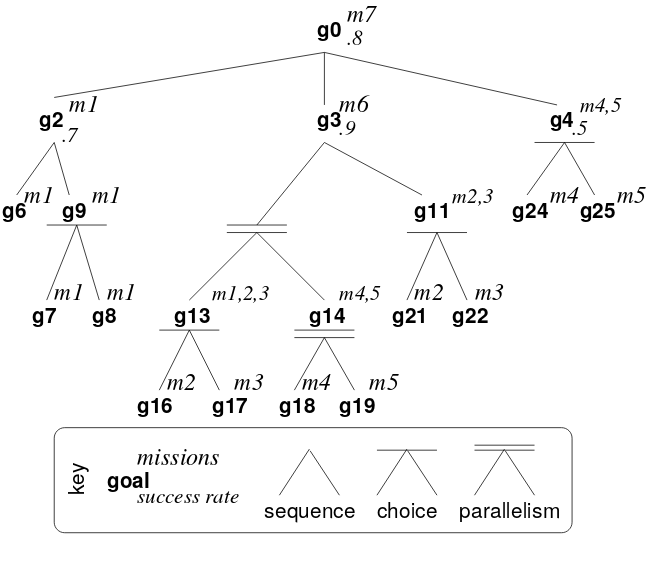
\includegraphics[width=0.8\linewidth]{figure/figmoise} 
  \caption{Arvore de objetivos definido pelo modelo Moise \cite{mosieframework}}
  \label{arvoremoise}
\end{figure}

A figura \ref{arvoremoise} define três tipos de relação de subobjetivos; $sequence$ onde todos os subobjetivos devem necessariamente ser concluídos em sequência, $choice$ onde o agente tem a 
possibilidade de escolher qual objetivo ele deseja seguir e $parallelism$ onde todos os objetivos devem ser concluídos, contudo sem uma sequência definida. Como é possível observar na figura, 
os objetivos são agrupados em conjuntos de missões $m$. A relação a seguir define isso melhor;

\begin{eqnarray}\nonumber
	m_k = \{ g_n,...,g_m\}
\end{eqnarray}


A Especificação Deôntica define predicados para estabelecer permissões e obrigações entre os papeis e as missões. Toda obrigação implica necessariamente em uma permissão. A relação a seguir 
estabelece isso; 

\begin{eqnarray}\nonumber
	obl(\rho,m,tc) \to per(\rho,m,tc) \\
	obl(\rho,m,tc) \wedge \rho \sqsubset \rho' \to obl(\rho',m,tc) \\
	per(\rho,m,tc) \wedge \rho \sqsubset \rho' \to per(\rho',m,tc) \\	
\end{eqnarray}

Onde o predicado $obl$ define uma obrigação e o predicado $per$ define permissão. O argumento $tc$ define uma periodicidade de tempo para o qual a relação deôntica é valida. 
